\section{Python Console}\label{pythonConsole}

Python Console

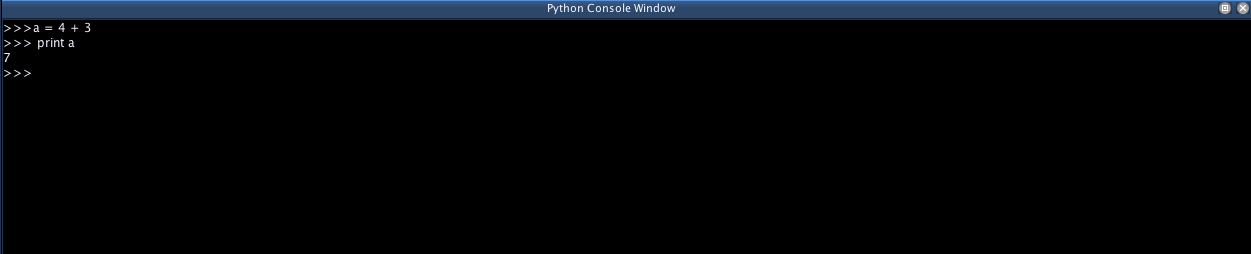
\includegraphics[width=1.00000\textwidth]{images/pythonConsole.png}

The Python Console allows you to interactively write and execute python
code using the Jython interpreter built in to blue. Because blue does
not clear the environment of the interpreter between runs, the console
can be useful to interactively inspect objects. Some ways you might use
the console:

\begin{itemize}
\tightlist
\item
  Use

  dir()

  to inspect objects to see what methods and members they have
\item
  Use

  help()

  to view the documentation on an object or class.
\item
  After generating a score or using the "Test" button on a PythonObject,
  you can interactively test functions you have written by calling it
  using code in the console.
\item
  Practice your python coding live.
\end{itemize}

The console works much like running python interactively in a console or
terminal. At the "\textgreater{}" prompt, you can type in some code,
then press enter to execute the code. All output from python functions
(including things like print statements in PythonObjects in the Score or
Python NoteProcessors) will output to the Python Console.

Some useful shortcuts available while in the console:

\begin{longtable}[]{@{}ll@{}}
\caption{Shortcuts for the Python Console}\tabularnewline
\toprule
Shortcuts & Description\tabularnewline
\midrule
\endfirsthead
\toprule
Shortcuts & Description\tabularnewline
\midrule
\endhead
ctrl-up/ctrl-down & cycle through previous commands used\tabularnewline
ctrl-l & clear the console (also available from the rt-click popup
menu\tabularnewline
\bottomrule
\end{longtable}
